\documentclass[11pt, oneside]{article} 
\usepackage{geometry}
\geometry{letterpaper} 
\usepackage{graphicx}
	
\usepackage{amssymb}
\usepackage{amsmath}
\usepackage{parskip}
\usepackage{color}
\usepackage{hyperref}

\graphicspath{{/Users/telliott/Github/precalculus/fig/}}
% \begin{center} \includegraphics [scale=0.4] {gauss3.png} \end{center}

\title{Basic geometry and congruen ce of triangles}
\date{}

\begin{document}
\maketitle
\Large

\subsection*{Euclid and the postulates}
Greek geometry starts hundreds of years before Euclid, who was a contemporary of Alexander the Great (356-323 BC).  

We know that Euclid lived after Plato (d 347 BC), and before Archimedes (b 287 BC).  Except that he worked in Alexandria, all other details of his life and death are shrouded in mystery.

After more than 2000 years, Euclid's book \emph{Elements} is still an excellent place to begin surveying the foundations of geometry.  It is a textbook, an organized collection of what was known about the subject at the time, or at least, everything that a well-educated student should know.

\begin{center} 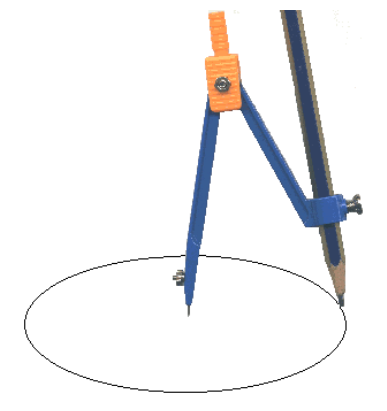
\includegraphics [scale=0.3] {compass.png} \end{center}

This book of consists of \emph{propositions}, which include constructions (geometric figures) drawn with a pencil on a piece of paper, using a straight-edge or a compass or both.  Often proofs of propositions build on previous items in the book.  Euclid does not prove everything.  Bertrand Russell was famously disappointed about that.

Here are Euclid's first three postulates --- statements that are assumed to be true:

$\bullet$  A straight line segment can be drawn joining any two points.

$\bullet$   Any straight line segment can be extended indefinitely in a straight line.

$\bullet$   Given any straight line segment, a circle can be drawn having the segment as the radius and one endpoint as the center.

Let us assume these as well.  We will use them often.

We finesse the difficulty in defining what is meant by \emph{straight} in the real world.  If you've ever done any carpentry, for example, you probably know that unknown edges are determined to be straight by comparison with a known straight edge.  We use an imaginary perfect straight-edge and draw a straight line as "the shortest distance between two points".

The fourth postulate is:

$\bullet$   All right angles are congruent, that is, equal to each other.

This one prompts a different question:  what is a \emph{right angle}?

If one line segment (piece of a line) is drawn crossing a second one, forming their \emph{intersection}, let us refer to the angles formed on the same side of a line as \emph{supplementary} angles (also sometimes called adjacent angles).

\begin{center} 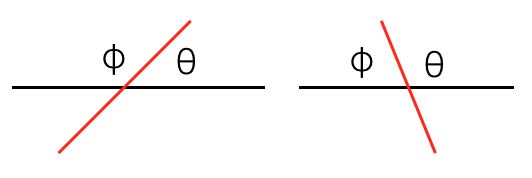
\includegraphics [scale=0.4] {lines_angles_1.png} \end{center}

On the left, one of the angles, $\phi$, is larger than the other one, $\theta$.  On the right, we have $\phi < \theta$.  

The third possibility is that $\theta = \phi$.  The definition of a right angle is that 

$\bullet$ \ if two supplementary angles are equal, they are both right angles.  

\begin{center} 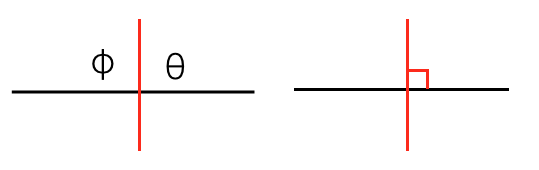
\includegraphics [scale=0.4] {lines_angles_2.png} \end{center}

A right angle is frequently designated by drawing a small square, as seen in the right panel above.

Regardless of whether $\theta < \phi$, $\theta > \phi$, or $\theta = \phi$, the sum of the two angles $\phi + \theta$ is equal to two right angles or 180 degrees.

There is nothing particularly special about using $90$ degrees as the measure of a right angle, $180$ degrees for any two supplementary angles including right angles, or $360$ degrees for one whole turn.

Well, there is one thing:  there are \emph{approximately} 360 days in a year, which marks the sun's track across the sky.  

In his book, \emph{Measurement}, Lockhart adopts the convention that a whole turn is equal to $1$.  

Later, we'll see that one whole turn can be defined using a different unit of measure as $2 \pi$ \emph{radians}, and that convention turns out to be quite important for calculus.

Now, consider those angles lying below the horizontal:

\begin{center} 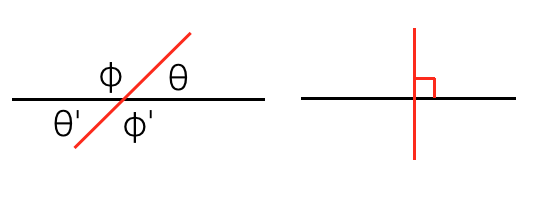
\includegraphics [scale=0.4] {lines_angles_3.png} \end{center}

We said that the sum of the two angles $\phi + \theta$ is equal to two right angles, but so are the sums $\theta' + \phi$ and $\theta + \phi'$, for the same reason.  As a result

\[ \phi + \theta = \theta + \phi' \]
We conclude that $\phi = \phi'$ and $\theta = \theta'$.  

This is called the \emph{vertical angle theorem}.

On the right, if any one of the angles where two lines cross is a right angle, then all four are right angles.

\subsection*{parallel postulate}

So far, all this seems rather obvious.  The fifth and final postulate is more subtle:

$\bullet$   If two lines are drawn which intersect a third in such a way that the sum of the inner angles on one side is less than two right angles, then the two lines inevitably must intersect each other on that side if extended far enough.

Line $1$ and line $2$ are parallel, if and only if, $A + C = B + D = 180 = 2$ right angles.

\begin{center} 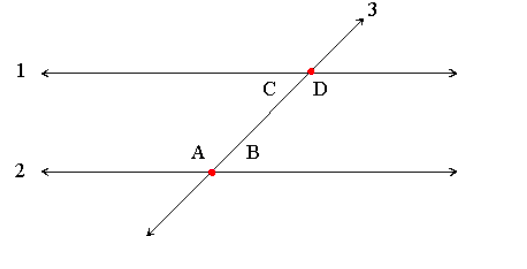
\includegraphics [scale=0.5] {alternate_interior_angles.png} \end{center}

This postulate is equivalent to what is known as the parallel postulate.

\url{http://mathworld.wolfram.com/EuclidsPostulates.html}

But we also know from the properties of two lines given above that the supplementary angles $A + B = 180$ add up to $180$ degrees. So
\[ A + C = 180 = A + B \]
and then
\[ C = B \]

This is called the theorem on \emph{alternate interior angles} between two parallel lines.

We note that adoption of this postulate is a choice.  The definition works for geometry in the flat plane.  

But, consider a familiar situation where this is not true.  Suppose we are doing geometry on the surface of a sphere, such as the earth.

Then, two adjacent lines of longitude can be drawn so as to cross the equator at right angles, and the lines are parallel there, but they will meet (intersect) at the poles.  

\begin{center} 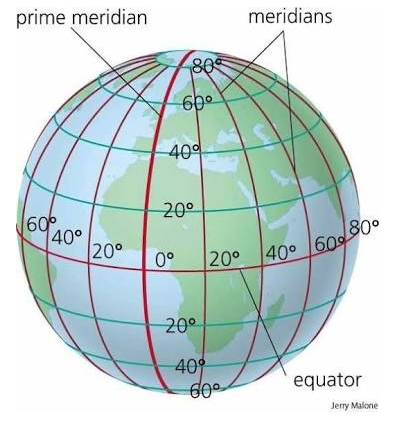
\includegraphics [scale=0.5] {lat_long.png} \end{center}

The parallel postulate only holds for geometry on a \emph{flat} surface.

\subsection*{axioms}

Euclid also lists five axioms, things which are assumed.  Here are two examples:

$\bullet$   Things that are equal to the same thing are also equal to one another.

$\bullet$   If equals are added to equals, then the wholes are equal.

These seem quite reasonable.

We will see how to proceed from the postulates and axioms to various proofs.  \emph{Given these assumptions}, we can prove theorems that must be true.

\subsection*{Thales}
I'm a big fan of William Dunham's books --- several of them are listed in the References.  

Dunham has written a lot about the history of mathematics in Greece, starting with Thales (624-546 BC), who was from a Greek town called Miletus on the coast of Asia Minor (modern Turkey).  He lived long before Euclid (about 300 years before, 600 BC).  Although none of his writing survives, it is believed that Thales proved several early theorems including one we saw above. 

$\bullet$  The vertical angles formed by two straight lines crossing, are equal.
\begin{center} 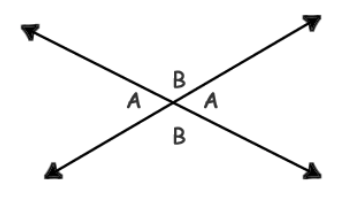
\includegraphics [scale=0.4] {vertical_angles.png} \end{center}

This theorem, which we already proved, depends on a property of straight lines.  In the proof, we used the axiom  "equals added to equals are equal", alternatively "equals subtracted from equals are equal."

A very important theorem attributed to Thales is the following:

$\bullet$  The angle sum of a triangle is equal to two right angles.
\begin{center} 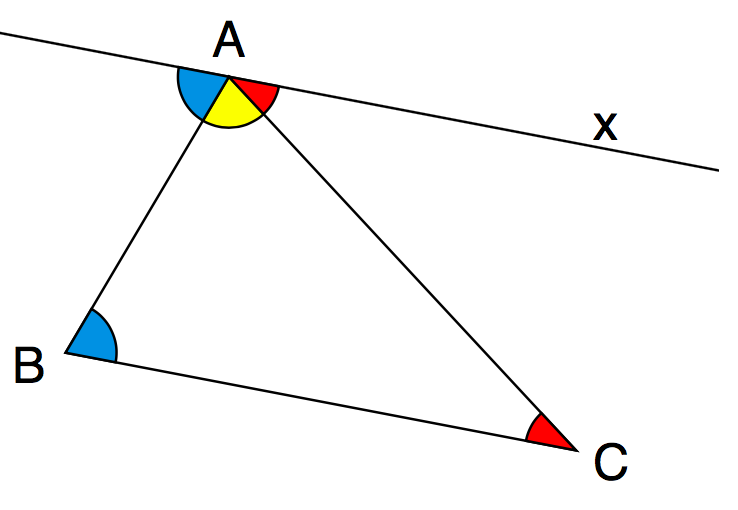
\includegraphics [scale=0.3] {triangle_sum_angles.png} \end{center}

This theorem depends on the ideas we developed above.  Draw a line segment through $A$ parallel to $BC$.  Now, use alternate interior angles and follow the colors to the result.

We will see one more theorem ascribed to Thales (it is actually called Thales' theorem), in the next chapter.  It is about isosceles triangles (two sides equal).

\subsection*{another proof}
Here is a different proof of the theorem on the sum of angles in a triangle adding to 180 degrees.  It never hurts to re-prove things by a different method.  It serves as a check on both the result, and the methods.

Imagine walking around the perimeter of a triangle in the counter-clockwise direction.  At each vertex we turn left by a certain number of degrees, $\theta$, called the exterior angle.  After passing through all three vertices, we must end up facing in the same direction as we started.

The sum of the exterior angles is $360^\circ$.

\begin{center} 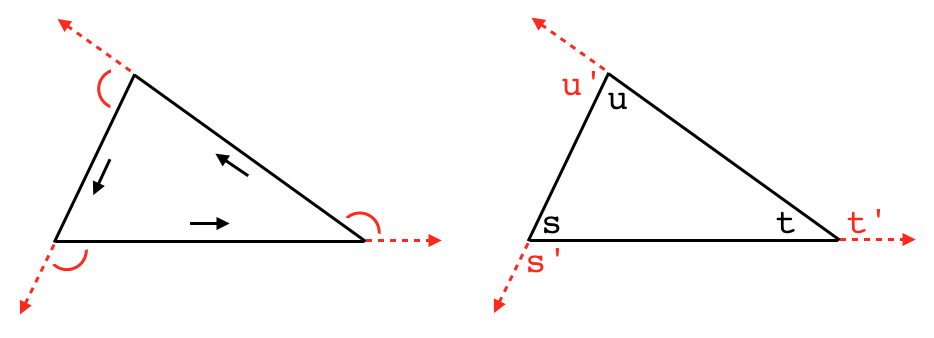
\includegraphics [scale=0.4] {lines_angles_trisum.png} \end{center}

\[ s' + t' + u' = 360 \]

In addition, for each vertex, the interior angle plus the exterior angle add up to $180$ degrees.  If we add all three pairs, we obtain
\[ (s + s') + (t + t') + (u + u') = 3 \cdot 180 = 540 \]
By subtraction
\[ s + t + u = 180 \]

\subsection*{summary}

Make sure you understand each of these theorems:

$\bullet$ \ supplementary angles

$\bullet$ \ vertical angles

$\bullet$ \ alternate interior angles

$\bullet$ \ triangle sum



\end{document}